\documentclass{article}
%%%%%%%%%%%%%%%%%%%%%%%%%%%%%%%%%%%%%%%%%%%%%%%%%%%%%%%%%%%%%%%%%%%%%%%%%%%%%%%%%%%%%%%%%%%%%%%%%%%%%%%%%%%%%%%%%%%%%%%%%%%%%%%%%%%%%%%%%%%%%%%
\usepackage{generalsnips}
\usepackage{enumitem}
\usepackage{url}
\packagesneeded
\usepackage[top=0.6in, bottom=1in, left=1in, right=1in]{geometry}
\title{Ensayo De Planeación- Apple Analysis}
\date{2020-Mar-02 22:03:00}
\author{David Gabriel Corzo Mcmath}
%%%%%%%%%%%%%%%%%%%%%%%%%%%%%%%%%%%%%%%%%%%%%%%%%%%%%%%%%%%%%%%%%%%%%%%%%%%%%%%%%%%%%%%%%%%%%%%%%%%%%%%%%%%%%%%%%%%%%%%%%%%%%%%%%%%%%%%%%%%%%%%
\begin{document}
\maketitle
%%%%%%%%%%%%%%%%%%%%%%%%%%%%%%%%%%%%%%%%%%%%%%%%%%%%%%%%%%%%%%%%%%%%%%%%%%%%%%%%%%%%%%%%%%
\section{Empresa que admiro: Apple}
Es una empresa que ha sido líder en el mercado de tecnología por un tiempo de por lo menos una década. Esta empresa hace unos meses llego a ser valorada en un trillón de dólares, es una empresa multinacional que aporta día a día mucho valor a sus consumidores.

%----------------------------------------------------------------------------------------

\subsection{FODA}
\begin{center}
   \begin{tabular}{ | p{8.25cm} | p{8.25cm} | }
        \hline
            \textbf{Fortalezas: } 
            \begin{itemize}
                \item Alta capacidad de gestionar problemas.
                \item Capacidad gerencial ágil.
                \item Capacidad de adaptarse bien al mercado.
                \item Capacidad de trabajar con diversos tipos de personas.
                \item Capacidad de innovar constantemente.
            \end{itemize}
            &
            \textbf{Oportunidades: } 
            \begin{itemize}
                \item Áreas que se están globalizando tienen alta demanda por dispositivos electrónicos fáciles de usar.
                \item A la gente le está atrayendo el ecosistema Apple que se obtiene al adquirir dispositivos con ellos.
                \item Hay un alto crecimiento en la tendencias por el uso de un teléfono móvil a el uso de una computadora. 
            \end{itemize}
            \\ 
        \hline
            \textbf{Debilidades: } 
            \begin{itemize}
                \item La empresa es muy grande y tiene problemas de competitividad con ciertas regiones del mundo.
                \item Los productos tienden a tener baja compatibilidad con productos competidores.
            \end{itemize}
            &
            \textbf{Amenazas: } 
            \begin{itemize}
                \item Impuestos en diversos lugares.
                \item Legislación gubernamental de cada región puede ser problemática para la empresa.
                \item Ciudad ambiente: los desperdicios tecnológicos preocupan a los clientes. 
                \item Coronavirus: muchas partes son creadas en China y la baja producción podría causar deficiencia en sacar el producto.
            \end{itemize}
            \\ 
        \hline
   \end{tabular}
\end{center}



%----------------------------------------------------------------------------------------
\subsection{Valores}

Los valores de dominio público de esta empresa son: 
\begin{itemize}
    \item Accesibilidad: productos fáciles de utilizar.
    \item Educación: servicios educativos fáciles de usar.
    \item Ambiente: proporciona un ambiente confiable a sus trabajadores.
    \item Inclusión y diversidad: un equipo de trabajo diverso.
    \item Privacidad: productos que no comprometen la seguridad del individuo.
    \item Ofertante responsable: un proveedor de productos que es confiable y no va a quedar mal.
    \item Integridad y responsabilidad con el cliente.
\end{itemize}

\subsubsection{Misión y visión}
\begin{itemize}
    \item Misión: ``to bringing the best user experience to its customers through its innovative hardware, software, and services.''
        \begin{itemize}
            \item ¿Quiénes somos?
                \begin{itemize}
                    \item Una empresa que se compromete con sus clientes a tener los mejores productos en términos de usabilidad y experiencia de usuario.
                \end{itemize}
                
            \item ¿Cuál es la promesa de servicio?
                \begin{itemize}
                    \item Facilidad, excelencia, experiencia de usuario inolvidable.
                \end{itemize}
                
            \item ¿Qué ofrecemos que nos hace únicos?
                \begin{itemize}
                    \item A comparación de la competencia tenemos una intefaz de usuario que nos hace únicos, además tenemos un sistema operativo prácticamente a prueba de virus, además todo es fácil de manipular y de hacer.
                \end{itemize}
                
            \item ¿Quiénes son nuestros clientes?
                \begin{itemize}
                    \item Todas las personas interesadas en productos de calidad que tengan grandes capacidades y sean fáciles de usar.
                \end{itemize}
                
        \end{itemize}
    
    \item Visión: ``This vision set in stone follows a few key and core believes: Making great products , Focusing on innovation , Simplicity in place of complexity , Control the primary technologie, behind Apple's products, Focus on a few key projects, Excellence as the standard''.
        \begin{itemize}
            \item \pregunta{Hacia dónde vamos} 
                \begin{itemize}
                    \item Mediante el enfoque en innovación están intentando ``complicarse ellos para que tu no tengas que complicarte''.
                    \item Excelencia.
                \end{itemize}
                
            \item \pregunta{En qué queremos ser un referente} 
                \begin{itemize}
                    \item Innovadores, excelencia en productos que sean fáciles de usar.
                \end{itemize}
                
            \item \pregunta{Cómo nos vemos en el futuro} 
                \begin{itemize}
                    \item Haciendo productos grandes.
                    \item Concentrandonos en innovación.
                \end{itemize}
                
            \item \pregunta{Cuál será nuestro legado} 
                \begin{itemize}
                    \item ``Simplicity in place of complexity'' dejar la corriente de hacer productos fáciles de usar que brinden al cliente poder.
                \end{itemize}
                
        \end{itemize}
\end{itemize}



%----------------------------------------------------------------------------------------
\subsection{Estrategia global de competencia}
\begin{itemize}
    \item La estrategia es diferenciación: dado a que respecto a sus competidores en el mercado tiende a sacar productos que se diferencian respecto a los de los demás, en términos de precio son significamente más caros que sus competidores y esto sólo por el hecho de ser la marca que son, sus productos son considerados por muchos un bien de status.
    \item Es notable cuál es su estrategia de producto o servicio ya que brindan bienes con mucho valor agregado, por otro lado a pesar que producen vasta cantidad de producto se tiende a considerar un producto que tiene muchos fans, ellos compran el producto no mas sale al mercado, e inicialmente siempre es escaso encontrar un producto apple cuando es muy nuevo.
    \item La estrategia de mercado es especialmente interesante también por el hecho que como son productos de status se dan cosas como ediciones especiales vendidas a un precio diferenciado respecto a sus competidores.
    \item La estrategia de ventas, Apple sólo distribuye sus productos a través de una cadena global de vendedores autorizados, estas son características medulares de un estrategia global de competencia de diferenciación.
    \item Estrategia global de competencia es además de diferenciación innovación, la innovación se ve claramente cuando Apple saca múltiples productos en un lapso relativamente corto.
\end{itemize}



%----------------------------------------------------------------------------------------
\section{Plazos de la planeación estratégica}
\begin{center}
    \begin{tabular}{ |p{4cm}|p{4cm}|p{8cm}| }
        \hline
            Plazo & Criterios & Justificación \\
        \hline 
            Corto plazo (1 año): 
            & 
            \begin{itemize}
                \item Periodo de recuperación de la inversión.
            \end{itemize}
            & 
            \begin{itemize}
                \item Dado a que Apple tiende a sacar productos con una demanda que se puede deducir con algún nivel de certeza inelástica el periodo en el que se recuperará la inversión es parte de la planeación estratégica a considerar a corto plazo.
            \end{itemize}
            \\ 
        \hline
            Mediano plazo (5 año): 
            & 
            \begin{itemize}
                \item Velocidad de cambio en la tecnología.
            \end{itemize}
            & 
            \begin{itemize}
                \item La velocidad de cambio es un factor influyente por el hecho que hay competidores y es más fácil posicionarse en el mercado si son los primeros en lanzar una nueva tecnología. También en términos de mantenerse al tanto, si no se mantiene al tanto de cómo progresa la tecnología y qué demandan sus clientes habrán pérdidas.
            \end{itemize}
            \\ 
        \hline
            Largo plazo (10 año): 
            & 
            \begin{itemize}
                \item Barreras de entrada y salida a nuevos mercados.
            \end{itemize}
            & 
            \begin{itemize}
                \item Dado a que las barreras de entrada a cada país son diferentes al Apple estar ya instalado en una vasta cantidad de países se puede deducir que se necesita conocimiento para especular cómo va a estar el mercado en 10 años, qué tan factible es salir, un ejemplo es Venezuela, hay que planear si se necesita salir o entrar a nuevos mercados.
            \end{itemize}
            \\ 
        \hline
    \end{tabular}
\end{center}


%%%%%%%%%%%%%%%%%%%%%%%%%%%%%%%%%%%%%%%%%%%%%%%%%%%%%%%%%%%%%%%%%%%%%%%%%%%%%%%%%%%%%%%%%%
\section{Fuerzas competitivas de Michael Porter}
Los dos componentes del análisis de las fuerzas competitivas de Michael Porter que he decido escoger han sido las de clientes y nuevos entrantes al mercado.

%----------------------------------------------------------------------------------------
\subsection{Clientes}
Los usuarios de los productos Apple a diferencia de varias empresas se catalogan en muchas categorías, entre estas categorías están grupos tan grandes como industrias. Apple tiene demanda de las siguientes grupos:
\begin{itemize}
    \item Ebay Inc. 
    \item Verizon Communications 
    \item Staples Inc. 
    \item Amazon com Inc. 
    \item Sprint Corporation 
    \item Etcétera
\end{itemize}

Esta empresa sirve desde empresas pequeñas hasta grandes conglomerados de empresas. A continuación una gráfica que muestra el crecimiento de Apple por cliente o industria en año 2019: 
\begin{center}
    \begin{figure}[htb]
        \centering
        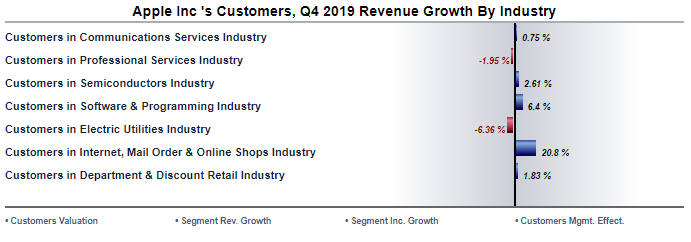
\includegraphics[width=10cm]{./figs/global.PNG}
        \caption{Apple Inc 's Customers, Q4 2019 Revenue Growth By Industry}
    \end{figure}
\end{center}
Como podemos observar Apple tiene como clientes a un gran conglomerado de empresas al igual que clientes directos que consumen sus productos, la demanda para sus productos es una de las más fuertes del mundo y es una tendencia que Apple ha seguido muy bien. El tamaño del mercado es grandísimo y además por haberse analizado esta fuerza se deduce que es un mercado altamente competitivo.


%----------------------------------------------------------------------------------------
\subsection{Competidores directos}
Ahora que existe Apple, que una empresa entre y que intente superar a Apple sería altamente difícil, es por eso que una fuerza competitiva más interesante de analizar son los competidores que Apple ya tiene. Samsung, Huawei entre otros son competidores directos de Apple, sirven también a grandes conglomerados de empresas y a clientes individuales. Uno de los competidores más grandes de Apple es Google y Microsoft, dado a que los dos son denominados ``tech giants'' en el mercado. Sin embargo lso productos de los competidores son diferentes y ofrecen diferente valor agregado, por Apple usar diferenciación al hacer el marketing de sus productos se aprecia que el cliente compra los productos y servicios por un valor agregado diferente al de la competencia, es por eso que los competidores directos y Apple tiene un mercado que se podría decir que buscan los productos y servicios tecnológicos pero que lso clientes de Apple buscan además que sus productos sean Apple por el valor agregado que les brinda.

\subsection{Conclusión}
Al haberse analizado las dos fuerzas anteriores se puede concluir con certeza que el mercado en el que opera Apple y sus competidores es altamente competitivo, dado a que el mercado es gigantesco. Además Apple tiene muchos competidores que se dedican a hacer productos y a brindar servicios de similar categoría. 
Se puede entonces decir que la posición en la matriz de posicionamiento del mercado esté en algún lugar en el primer cuadrante dado al precio alto y a la alta calidad. 

%%%%%%%%%%%%%%%%%%%%%%%%%%%%%%%%%%%%%%%%%%%%%%%%%%%%%%%%%%%%%%%%%%%%%%%%%%%%%%%%%%%%%%%%%%
\section{Fuentes}
\begin{itemize}
    \item \url{https://fourweekmba.com/apple-mission-statement-vision-statement/}
    \item \url{https://www.apple.com/}
    \item \url{https://www.apple.com/newsroom/2017/11/the-facts-about-apple-tax-payments/}
    \item \url{https://csimarket.com/stocks/markets_glance.php?code=AAPL}
    \item \url{https://www.owler.com/company/apple}
\end{itemize}





\end{document}
